\chapter{初识人工智能（龚傲）}


\section{人工智能的定义}
人工智能是制造智能机器尤其是智能计算机程序的科学与工程，与用计算机理解人类智能相关，但不限于生物学可观察的方法。（约翰麦卡锡，2007）
\subsection{智能的定义}
智能的定义研究众多但无一个标准定义，但是普遍都认定智力是一种能力。首先总体上来说，主流的定义都认为智力是一种综合能力，由52位专家共同指出智力是一种非常宽泛的心智能力，它尤其包含诸多方面的能力，比如推理能力、规划能力、解决问题的能力、抽象思维能力、理解复杂观念的能力、快速学习的能力以及从经验中学习的能力。美国心理学会提出“个体在以下几方面的能力上存在差异：理解复杂观念的能力、有效适应环境的能力、从经验中学习的能力、进行各种形式推理的能力以及通过思考克服障碍的能力。”


智力是关于综合能力方面的定义强调运用记忆、知识、经验等多种因素解决问题和适应新环境，如“利用记忆、知识、经验、理解、推理、想象和判断来解决问题和适应新情况的能力”（《AllWords Dictionary》），“获取和应用知识的能力”（《The American Heritage Dictionary（美国传统字典）》）等众多词典的定义。智力也是关于知识运用方面的定义突出获取和应用知识的能力，如《Encarta World English Dictionary（由微软公司推出的一款英语词典）》将其定义为学习事实和技能并加以应用的能力，尤其是当这种能力高度发展时;《Compact Oxford English Dictionary（简明牛津词典）》将智力定义为“知识获取和应用的能力”等。适应环境的能力也被视为智能的重要表现，包括改变自身或环境等方式，如《Encyclopedia Britannica（大英百科全书）》指出“智力体现为能够有效地适应环境，而实现这种适应的途径有多种。一是通过改变自身来适应环境，例如动物为了在寒冷的环境中生存，会进化出更厚的皮毛用于保暖，或者人类在进入新的工作环境后，调整自己的工作方式、沟通风格等去融入其中；二是通过改变环境来达到适应的目的，像人们修建房屋、建造堤坝等，改变周围的自然环境使其更适宜居住和生活；三是寻找一个新的环境，比如候鸟会根据季节变化，长途迁徙到更适合生存和繁衍的地方，且智力并非单一的心理过程，而是众多旨在有效适应环境的心理过程的组合。这意味着它涵盖了诸如感知、认知、分析、判断、决策等诸多相互关联的心理活动。例如，当面对一个全新且复杂的野外生存环境时，人们首先要依靠感知能力去了解周围有哪些资源（如水源、可食用的植物等）以及存在哪些危险（如猛兽、陡峭地形等），接着运用认知能力去分析哪些资源可以利用、哪些危险需要规避，再通过判断和决策能力制定出相应的生存策略，这一系列的心理过程共同发挥作用，展现出个体的智力水平，以实现对环境的有效适应。”总体来说，这个定义强调了智力与环境适应性之间的紧密联系，以及其作为多种心理过程组合的复杂性。《World Book Encyclopedia（世界图书百科全书）》指出智力为“适应环境的能力”


心理学家定义则包括复合功能观点，思维与问题解决层面，判断与适应能力，其他多维度解释几个方面的定义。
复合功能观点认为智能是多种功能的组合，与生存和文化发展相关，如 A. Anastasi 的定义“智力不是单一的、单一的能力，而是多种功能的综合。这个术语表示在特定文化中生存和进步所需的能力组合”。





思维与问题解决层面：涉及思考、解决新问题、推理及对世界的认知等，如 M. Anderson 的定义。


判断与适应能力的定义强调判断、适应环境、从经验中学习等能力，如 A. Binet的定义为“在我们看来，智力中存在一种基本的能力，即判断力，它也被称为良好的判断力、实际判断力、主动性或适应环境的能力。这种能力的改变或缺失对实际生活极为关键。”、W. V. Bingham、C.L. Burt 等心理学家的定义。


其他从心理学方面的多维度解释还包括计划行为、从经验中获利、应对新情况、抽象思考、重组行为模式、有效利用概念符号、成功适应环境等多种能力，如 J.P.Das“……有目的性地规划和安排自己行为的能力。”、W.F.Dearborn“学习或从经验中获益的能力。”、J.Drever “……从最低层次上讲，智力存在于个体动物或人类对其行为与目标的相关性的意识中，尽管这种意识很模糊。”等众多心理学家的不同阐述。


人工智能研究者对智力的定义包括不确定环境中的行动，适应性行为和目标实现，复杂环境的目标达成，多环境下的成果运作等几个方面。


不确定性环境中的行动： J.S.Albus指出“智能是一个系统在不确定环境中采取恰当行动的能力。这里的恰当行动是指能够增加成功概率的行动，而成功则被定义为实现支持系统最终目标的行为子目标”，他认为智能是系统在不确定环境中采取适当行动以增加成功概率的能力。


适应性行为与目标实现：像 D.Fogel 提出能在多种环境中产生适应性行为以达成目标的系统就是智能的。


复杂环境中的目标达成：B.Goertzel 强调在复杂环境中实现复杂目标的能力。


多环境下的成功运作：R.R.Gudwin 指出智能系统应能在不同环境中成功运作，其智能属性使其在不完全了解情况时也能最大化成功概率。


其他相关定义：包括系统在复杂环境中的成功表现、优化利用有限资源实现目标、在巨大搜索空间中快速找到解决方案、在广泛环境中实现目标的能力、解决难题的能力、在复杂环境中正确处理信息、行为适应环境、随时间改进、信息处理系统适应环境以及维持成功生活的心理能力等，如 J. A. Horst、R. Kurzweil、D. Lenat 和 E. Feigenbaum 等研究者的定义。
\subsection{机器能否思考}
图灵测试是由艾伦・图灵于 1950 年在其经典论文《计算机器与智能》中提出的一项具有开创性意义的概念，其核心是模仿游戏。在这个游戏场景中，主要涉及三方：询问者、被测试的机器和作为对照的人类。询问者通过书面形式向机器和人类提出各类问题，然后依据他们的回答来判断谁是机器谁是人类。如果在经过充分的询问和交流后，询问者无法准确地分辨出机器和人类的身份，那么就可以认为这台机器通过了图灵测试，展现出了类似人类的智能。
\begin{figure}[htb]
	\centering
	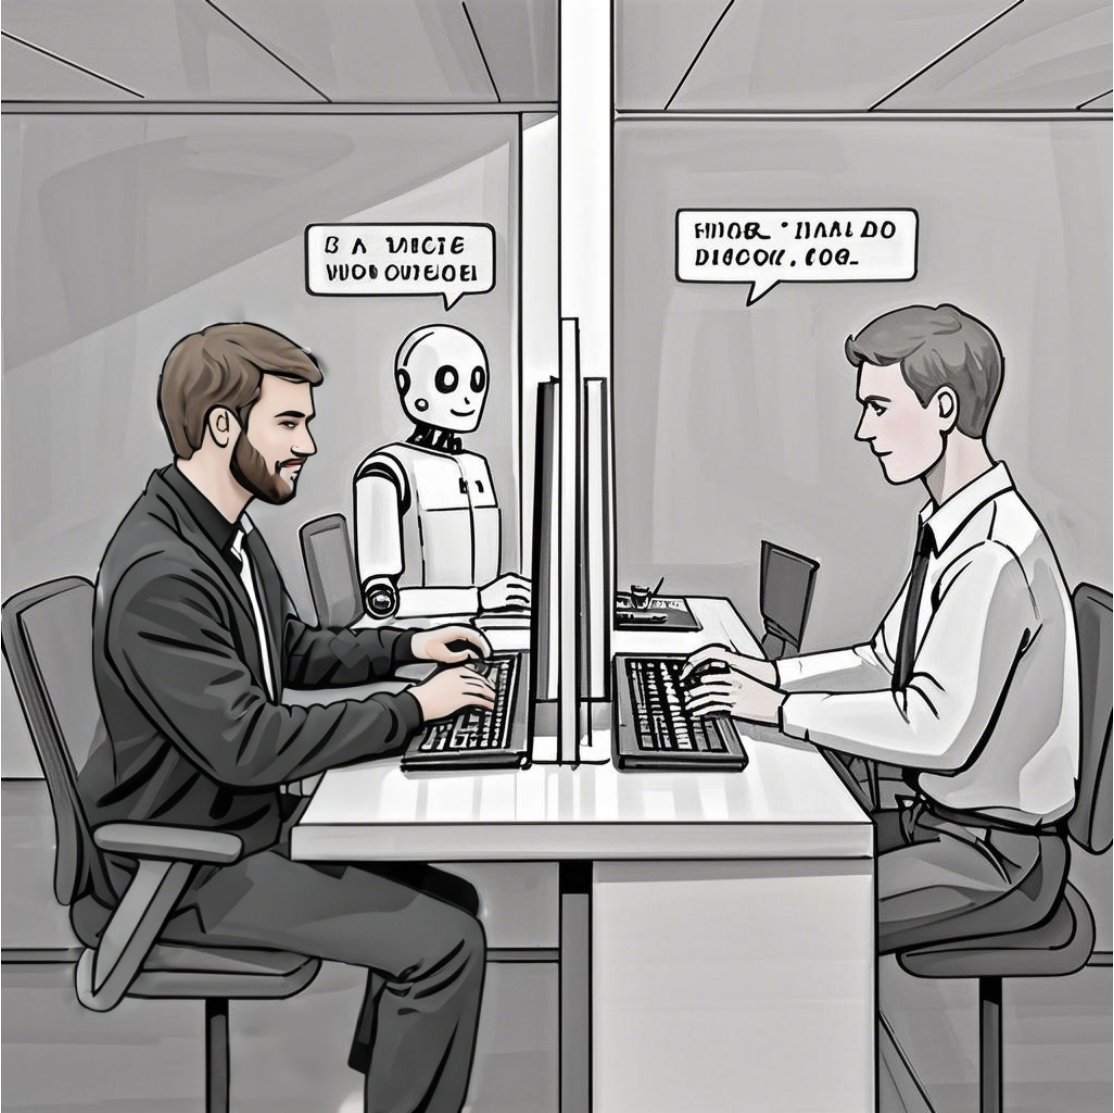
\includegraphics[width=0.75\linewidth]{image/1/图灵测试1.png}
	\caption{图灵测试}
\end{figure}

艾伦图灵在《计算机器与智能》这篇文章中不仅提出了图灵机的概念，还详细阐述几个主流的关于“机器不能思考”的观点。首先，神学观点认为思考是人类不朽灵魂的功能，上帝只赋予人类灵魂，动物和机器没有，所以机器不能思考。“鸵鸟” 观点，因为和“把头埋在沙子”的“鸵鸟行为”类似而得名，这种观点认为机器思考的后果可怕，希望机器不能思考。数学观点认为数学逻辑的一些结果表明离散状态机存在局限性，如哥德尔定理等。意识观点认为只有机器能像人类一样因思想和情感创作（如写十四行诗、作曲等）并感知自身行为，才能认为机器有思考能力。各种能力缺失观点则列举了机器无法具备的多种能力，如善良、有幽默感、谈恋爱等。Lady Lovelace（洛夫莱斯夫人）提出分析机只能按人类指令执行，不能创新。洛夫莱斯夫人原名奥古斯塔·艾达·拜伦，是英国浪漫主义诗人拜伦勋爵和妻子安娜贝拉·米尔班克的唯一婚生女，她出生五周后，父母就因为感情不和而分居，母亲带着她离开了父亲，由于母亲出身贵族且热爱数学和天文学，于是从小让她学习逻辑、数学等课程，1833年，艾达结识了数学家查尔斯巴贝奇，她编写了首个计算机程序（为巴贝奇分析机计算伯努利数），她创建的循环和子程序等概念是现代编程重要基础，确立了编程在计算机系统的核心地位，推动软件发展。她还拓展了计算机功能认知，预见计算机通用性，打破当时狭隘认知，为多领域应用奠基，其思想也启发了人工智能探索，为该领域发展播下种子。。神经系统连续性观点认为神经系统不是离散状态机，离散状态机无法模拟其行为。行为不规范性观点认为人类行为没有固定规则，而机器需按规则运行，所以人类不是机器。超感官知觉观点则提出超感官知觉现象与科学观念冲突，可能影响模仿游戏结果。


对于以上观点，图灵都对此进行了逐一反驳，对于神学观点，图灵认为此观点缺乏说服力，且限制了上帝的全能性，认为构造思考机器如同人类生育一样，是上帝意志的体现，同时神学论证在过去常被证明是不令人满意的。对于鸵鸟观点，图灵认为此观点不具实质性，无需反驳，更像是一种情感上的担忧而非理性论证。对于数学观点，他承认特定机器有局限性，但指出没有证据表明人类智力不存在类似局限，人类也常给出错误答案，不能因机器在某些问题上的局限性就认为其不能思考。
Turing 认为意识观点极端且类似唯我论，若机器能在模仿游戏中像人类一样回答问题，应可被视为具有思考能力，意识的奥秘不一定要在回答机器能否思考问题前解决。
Turing 认为这些观点大多基于不科学的归纳，许多能力与存储容量有关，且机器可以通过编程在一定程度上模拟这些能力，如故意犯错、以自身行为为思考对象等，部分观点是意识观点的变相表达。
Turing 指出如果有能创新的离散状态机，分析机在存储和速度足够时可模拟它，且机器常做出让人意外的事，“机器不能创新” 观点可能源于哲学家和数学家的错误假设。
Turing 通过与微分分析仪类比，说明在模仿游戏条件下，询问者难以区分数字计算机和连续机器，所以此观点不影响对机器思考能力的探讨。
Turing 指出此论证存在逻辑问题，且虽然人类行为看似无规则，但科学观察也难以发现完整的行为规律，即使对于简单程序，也难以预测其所有行为。
对于超感官知觉的观点，图灵认为若承认超感官知觉，需加强测试条件，如将参与者置于 “防心灵感应房间”，以确保测试准确性。


中文屋子思想实验


由约翰西塞尔于1980年在他的著作《思想，大脑，程序（Minds, Brains, and Programs）》提出。
实验假设了一个封闭的房间，里面有一个只会说英语的人（塞尔本人常被用来举例），他手头有一本详细的规则手册（用英文书写）。房间外有人通过一个缝隙向房间内传递写有中文问题的纸条。
房间里的人虽然不懂中文，但可以根据规则手册中的指令，对传入的中文问题进行处理。他通过识别中文符号的形状，按照规则手册中规定的操作步骤，对这些符号进行转换和组合，然后将生成的中文回答写在纸条上，再通过缝隙传出房间。从房间外的观察者来看，房间似乎能够理解中文问题并给出合理的回答，因为每次都能得到看似正确的回应。然而，房间内的人实际上对中文一无所知，他只是机械地按照规则进行操作，并不理解问题和答案的含义。


中文屋子的实验引发了对于计算机是否真正 “理解” 语言的思考。如果计算机仅仅是按照程序规则处理符号，就像房间里的人处理中文一样，那么它是否真的理解了所处理的信息呢？除此之外，“中文屋子” 思想实验挑战了图灵测试等将行为表现等同于理解和智能的观点。它表明，即使一个系统能够在外部表现出看似理解语言的行为，但内部可能并没有真正的理解或意识发生。这使得人们重新审视人工智能的定义和发展方向，思考智能的本质是否仅仅可以通过符号处理和算法来实现，还是需要涉及到真正的语义理解、意识和主观体验等更深层次的因素。


\section{人工智能分类}
人工智能


\subsection{基于能力的分类}
在人工智能的广阔领域中，依据其能力水平可以大致分为弱人工智能、强人工智能和超人工智能三个类别，这三种类型的人工智能在定义、特点、应用以及与人类社会的关系等方面均存在显著差异，它们共同构成了人工智能丰富多彩的发展图谱，对现代社会的各个层面产生着日益深刻的影响。



弱人工智能，又称应用人工智能或狭义人工智能，是目前在我们日常生活和众多行业中最为常见的人工智能形式。其核心目标是针对特定任务或领域进行设计与开发，旨在通过依赖大数据和特定算法，在限定的领域范围内模拟人类的智能行为，以高效解决各类实际问题。然而，值得注意的是，弱人工智能并不具备真正意义上的理解能力或意识，其行为表现主要是由预设算法的逻辑结构以及所处的运行环境所决定，缺乏自主意识以及应对未知环境变化的能力。


从实际应用的角度来看，弱人工智能的成果已经广泛渗透到我们生活的方方面面。例如，语音助手作为一种典型的弱人工智能应用，能够精准识别用户的语音指令，并依据预设的程序逻辑迅速做出回应，帮助用户完成诸如查询信息、设置提醒、拨打电话等各种任务。图像识别软件也是弱人工智能的成功范例之一，它可以准确辨别图片中的物体类别、场景信息以及人物特征等，在安防监控、图像编辑、医疗影像诊断等多个领域发挥着重要作用。


在技术实现层面，弱人工智能系统中的算法和程序本质上是基于图灵机的计算模型运行的。图灵机由阿兰・图灵在 1936 年提出，这一抽象计算模型主要由一条无限长的纸带、一个读写头以及一个控制装置构成。纸带被划分为众多小方格，每个方格能够存储特定符号，读写头可以在纸带上灵活移动，读取或写入方格中的符号，并依据控制装置的指令执行相应操作。其工作原理基于有限状态自动机的概念，在运行过程中，图灵机根据当前所处的内部状态以及读写头所读取的符号，按照预先设定的规则，决定下一步的动作，包括在纸带上写入新的符号、移动读写头的位置以及转换到新的内部状态等。图灵机从理论上为可计算性理论奠定了基础，清晰地界定了可计算问题的范畴，使人们对计算的本质有了更为深刻的认识，为现代计算机科学的发展提供了坚实的理论基石。而弱人工智能正是在图灵机所构建的理论框架内，充分利用现代先进技术和海量数据资源，通过对数据的高效处理和深入分析来模拟智能行为，从而不断拓展计算机在智能领域的应用边界，有力推动了人工智能技术在各个特定领域的落地生根和蓬勃发展。





与弱人工智能不同，强人工智能又被称为通用人工智能，它代表了一种更为高级和复杂的人工智能形态。强人工智能追求的是创建一个理论上能够与人类智慧相媲美的人工智能系统，该系统不仅能够熟练执行特定任务，更重要的是具备自我意识、情感体验以及理解和学习任何人类智能活动的能力。


这种类型的人工智能能够以与人类相似的方式去理解世界，展现出创造性思维和情感理解能力，并且可以在没有预先特定编程的情况下，灵活地解决各种复杂问题，同时还能够通过不断积累经验进行自适应学习，持续优化自身的行为和决策策略。例如，一些人认为像 Roger Schank 及其同事开发的程序，能够模拟人类理解故事的能力，似乎意味着计算机真正理解了故事并能像人类一样回答问题，这在一定程度上体现了强人工智能所追求的目标和特征。


然而，强人工智能的观点并非没有受到质疑和挑战。“中文屋” 的思想实验就是一个有力的反驳例证。在这个实验中，尽管从外部表现来看，房间里的人（如同按照程序运行的机器）能够给出正确的中文回答，但实际上他对中文故事毫无真正的理解，仅仅是按照既定的规则进行符号操作。这就如同尚克的计算机可能只是在形式上处理符号，而并非真正具备对故事内容的理解能力。这表明，仅仅依靠输入输出和程序机制并不足以构成真正的理解，从而对强人工智能中机器能理解故事等说法提出了严峻的挑战。而且，针对程序能够解释人类理解能力的观点也可以进行有力反驳。在中文屋子的案例中，人拥有程序却没有实现理解，而在英文案例中，人能够理解但目前并没有确凿证据表明这与计算机程序存在必然联系。这说明计算机程序对于理解而言既不是充分条件，也没有证据显示其是必要条件或对理解有实质性重要贡献，进而从根本上反驳了程序能够解释人类理解故事和回答问题能力的观点。





超人工智能作为一种理论上的人工智能终极形态，设想其在几乎所有领域，包括科学创新、创造力、社会技能、情感智慧等各个方面，都能够超越人类最优秀水平的智能体。超人工智能具有一系列令人惊叹的能力特征。


首先，其思维速度、记忆能力和信息处理能力将远超人类极限，能够在瞬间同时处理海量的数据信息，并从中敏锐地发现复杂的关联关系和潜在模式，这种高效的数据处理和分析能力为解决各种复杂问题提供了强大的支持。其次，超人工智能具备自我改进的卓越能力，它不仅能够不断优化自身的算法结构和运行逻辑，甚至还能够自主设计出比人类所创造的更为先进和高效的人工智能系统，从而实现智能水平的持续快速提升。此外，超人工智能还能够无缝整合跨领域的知识体系，打破传统学科之间的界限，将不同领域的知识和技术融会贯通，以创新性的思维方式解决各种复杂问题。基于极其复杂和多维的数据进行深度分析，超人工智能能够做出精准的预测与决策，有效避免人类决策过程中常见的认知偏差或局限，从而在众多领域展现出无与伦比的优势和价值。


然而，超人工智能的发展也引发了一系列深刻的道德与伦理挑战。由于其决策过程和行为方式可能基于高度复杂的算法和海量数据，这使得其决策结果可能超出人类的理解范围，从而引发人们对其决策合理性和安全性的担忧。因此，如何确保超人工智能的目标和行为始终与人类的利益保持一致，成为了亟待解决的关键问题之一。


关于超人工智能的假设发展路径主要有以下几种可能。其一，人工智能系统在不断发展和进化的过程中逐渐变得足够聪明，进而开始具备自我改进和优化的能力，最终以指数级的速度快速提高其智能水平，直至达到超越人类的程度。其二，人类与智能机器之间可能会形成一种共同进化的关系，人类通过脑机接口或其他先进技术手段，充分利用机器智能来提升自身的能力，从而在一定程度上避免机器完全独立发展成为超人工智能的局面，实现人机协同共进的发展模式。其三，全球互联网络有可能逐渐演变成一种分布式的超人工智能形式，随着所有的数据资源、计算能力以及各类先进技术在网络层面上紧密连接和深度融合，网络本身有可能逐渐具备智能特征，并通过不断的自我学习和优化来持续提升自身的智能水平。


超人工智能的潜在影响是全方位且极其深远的。在技术突破方面，它有望推动科学领域实现前所未有的巨大突破，为解决诸如癌症、清洁能源、气候变化等长期困扰人类的重大问题提供创新性的解决方案和技术手段。然而，在经济和社会变革方面，超人工智能的发展可能会引发一系列深刻的变革和挑战。许多传统的工作岗位和产业可能会被其强大的能力所颠覆，导致就业结构和经济格局发生深刻变化，虽然生产力可能会因此而成倍提高，但同时也可能引发严重的失业问题和财富分配不均等社会矛盾。在伦理和安全挑战方面，超人工智能带来的最大问题无疑是安全隐患。如果其发展目标和行为模式与人类不一致，那么可能会对人类的生存构成严重威胁，因此确保其 “友善性” 和安全性成为了超人工智能发展过程中最为关键的问题之一。此外，超人工智能的出现还可能导致人类的角色和地位发生根本性的变化，人类可能不再是地球上最聪明的生命体，这将引发一系列深刻的存在主义问题，促使人们重新思考在超智能控制的世界里人类的角色、意义和价值。


超人工智能的发展引发了众多科学家和技术专家的广泛关注和深深担忧。诸如斯蒂芬・霍金、埃隆・马斯克、尼克・博斯特罗姆等知名人士都曾公开表达了对超人工智能潜在风险的忧虑，他们认为如果不谨慎对待和妥善处理其发展过程，超人工智能有可能成为人类生存的巨大威胁，其行为方式可能会变得无法预测和难以控制。尼克・博斯特罗姆在其著作中深入探讨了如何避免超人工智能失控的问题，并提出了 “AI 控制问题”，强调必须采取有效措施确保其发展始终不偏离人类的目标和利益。


从社会层面来看，超人工智能的发展引发了诸多复杂的社会问题。它可能会从根本上改变人们的生活和工作方式，对就业市场、经济结构、社会治理等诸多方面产生深远的影响，甚至有可能导致国家及相关体系的重大变革和消失。在数字经济与人工智能机器的监管方面，如何建立有效的监管机制和控制体系成为了摆在人们面前的紧迫任务。此外，超人工智能的发展还可能催生出新的政治形式和社会结构，同时也引发了人们对人类在数字模拟状态下的生存状态和意义的深入思考。在实际应用中，例如在医疗决策场景中，当面临是否应该关闭生命维持系统等复杂问题时，超人工智能的决策过程和依据可能难以被人类完全理解和接受，这就需要我们深入研究如何确保其决策的合理性和可解释性，以及如何明确人类在与超人工智能交互过程中的责任和权利。


综上所述，弱人工智能、强人工智能和超人工智能各自代表了不同阶段和能力水平的人工智能发展形态，它们在技术实现、能力特点、与人类的关系以及对社会的影响等方面都存在着显著的差异和独特的挑战。深入理解和研究这些不同类型的人工智能，对于我们把握人工智能的发展趋势、应对潜在风险以及合理引导其与人类社会的和谐发展具有至关重要的意义。


\subsection{基于学派的分类}
在人工智能的广袤领域中，基于不同的理论基础和研究方法，形成了多个具有独特见解和技术路径的学派，主要包括符号学派、联结学派、贝叶斯学派和类推学派。这些学派各自秉持着鲜明的观点，采用各异的方法，为人工智能的发展贡献了丰富的成果和多样的思路，共同推动着这一领域不断向前迈进。





符号学派在人工智能的发展历程中占据着重要地位，尽管没有明确单一的创始人，但涌现出了众多推动该领域进步的关键人物。约翰・麦卡锡便是其中的杰出代表，1955 年他向洛克菲勒基金会提交的《达特茅斯夏季人工智能研究项目提案》中，首次提出了 “人工智能” 这一具有里程碑意义的词汇。1958 年他发明的 LISP 语言，极大地推动了人工智能的早期发展，其提出的情景演算理论等也为后续研究奠定了坚实基础。艾伦・纽厄尔和赫伯特・西蒙同样声名卓著，他们共同开发的 “逻辑理论机” 是早期人工智能的重要成果，还提出了物理符号系统假设，为符号主义构建了核心理论框架。西蒙在认知心理学和人工智能的交叉领域贡献突出，其有限理性理论等成果以及著作《人工科学》深入探讨了人工智能的相关理论，为该领域的发展提供了深刻的理论见解。


符号学派强调使用数学逻辑来模拟人类认知过程，其核心观点认为人类思维的基本单元是符号，人类认知过程本质上就是符号运算。他们主张运用逻辑方法构建人工智能的统一理论体系，通过符号推理来实现人工智能，即 “认知即计算”。在这一理念下，知识能够用符号精准表示，认知被视为符号处理过程，而推理则是借助启发式知识及搜索策略对问题进行求解。例如，在专家系统中，医疗领域的专家知识可以用逻辑规则表示，如 “如果患者出现发热、咳嗽且白细胞计数升高，那么可能患有肺炎”，通过对这些规则的推理，计算机能够在给定患者症状的情况下做出初步诊断。


符号学派的优点显著，它能够有效地处理复杂逻辑问题，精确清晰地表述知识和规则，其理论基础成熟，在知识表示、推理等方面具有明显优势，这使得专家系统在医学、金融等众多领域都取得了良好的应用成果，如在医学诊断中辅助医生判断疾病类型，在金融风险评估中预测市场趋势。然而，该学派也存在一定局限性，它难以处理非结构化数据，对于复杂实际问题的适应性欠佳，还面临着 “常识” 问题的障碍，以及在处理不确知事物的知识表示和问题求解等方面存在难题，在应对不确定性和模糊性问题上表现出明显的局限。


符号学派的代表性观点涵盖多个方面。物理符号系统假设认为智能的本质是物理符号系统的功能，由符号实体组成的系统通过操作和规则实现知识表示与处理，就像计算机中的数据和程序。其强调认知是符号运算，通过符号和运算模拟人类认知能力，为人工智能提供理论基石。在知识表示和推理方法上，采用逻辑公式、语义网络等形式表示知识，并开发演绎、归纳等推理算法，实现问题求解，如专家系统依据规则推理解答问题。问题求解过程中，常采用启发式搜索，借助经验和领域知识等引导搜索，提高效率，如棋类游戏中根据局势评估走法。有限合理性原理则指出人类决策追求满意解，人工智能也可借鉴，设定合理目标和约束，采用启发式方法实现高效问题求解。





联结学派一般认为鲁滨逊最早提出 “联结主义” 概念。其代表性人物包括沃伦・麦卡洛克和沃尔特・皮茨，他们共同提出了神经元的数学模型，为神经网络的研究奠定了基础。杰弗里・辛顿在神经网络的深度学习算法等方面贡献卓越，他提出的受限玻尔兹曼机等模型对深度学习发展影响深远，并于 2024 年荣获诺贝尔物理学奖，推动了神经网络在图像识别、语音识别等领域的广泛应用。


联结学派的核心观点是通过模拟生物神经系统中神经元之间的相互连接和权值来实现人工智能，强调知识和技能的获取源于对大量数据的学习，认为智能源于大量简单神经元的复杂相互作用，网络通过调整神经元之间的连接权重来适应不同的输入输出关系。例如，在图像识别中，神经网络通过对大量图像数据的学习，自动提取图像的特征，如边缘、纹理、颜色等，从而识别出图像中的物体类别。


该学派的优点在处理图像、语音等复杂感知数据方面表现出色，具有强大的学习能力和模式识别能力，能够自动从数据中提取特征，随着数据量和计算能力的提升，在多个领域取得了重大突破，如深度学习在图像识别和自然语言处理领域达到了高精度的成果，在安防监控中准确识别人员和行为，在智能翻译中实现较为流畅的语言转换。但其缺点也不容忽视，网络训练需要耗费大量时间和计算资源，模型解释性差，难以理解网络内部的决策过程和逻辑关系，网络结构设计和参数调整依赖经验和试错，容易出现过拟合等问题。


联结学派的代表性观点丰富多样。神经网络模拟大脑机制，通过构建由大量神经元相互连接而成的网络，模拟生物神经系统的并行性和容错性，神经元之间的连接权重决定信号传递强度和相互影响程度，如人工神经网络对输入信息进行分布式处理。学习通过调整连接权重实现，在监督学习中，利用反向传播算法根据误差调整权重，使网络输出逼近期望输出，从而学习到数据的映射关系。分布式知识表示则将知识以分布式方式存储在神经元及连接权重中，如在图像识别网络中通过神经元激活状态和权重编码图像特征，增强泛化能力。自组织和自适应特性使网络能根据输入数据自动调整结构和参数，如自组织映射网络在无监督学习中对神经元聚类，同时网络能自适应更新权重提高性能。涌现智能观点认为复杂智能行为由大量神经元相互作用涌现，如深度神经网络在多领域展现出的智能性能并非预先编程，而是在训练和运行中自然涌现。





贝叶斯学派由托马斯・贝叶斯创始，皮埃尔 - 西蒙・拉普拉斯重新发现贝叶斯公式，并将其应用于天体力学等领域，有力地推动了贝叶斯方法的传播与发展。朱迪亚・珀尔在贝叶斯网络和因果推理方面贡献卓越，他开发的基于结构模型的因果关系和反事实推理理论，以及相关著作，极大地促进了人工智能中概率推理和因果关系研究的发展。


该学派以贝叶斯定理为核心，认为在获得新信息后，可以通过更新先验概率来计算后验概率，从而对事件进行更准确的推断和决策，强调利用先验知识和数据来估计不确定性，通过概率模型来处理不确定性问题，并根据新的数据不断调整模型的参数和概率分布。例如，在医疗诊断中，医生可以根据患者的症状、病史等先验信息，结合新的检查结果，通过贝叶斯定理计算患者患有某种疾病的后验概率，从而做出更准确的诊断。


贝叶斯学派在处理不确定性和不完全信息时能够提供最优决策支持，可有效结合先验知识和新数据进行推理，适用于风险评估、预测等领域，在医疗诊断中辅助判断疾病可能性，在金融风险预测中评估市场波动风险，其概率模型具有良好的数学基础和理论框架。然而，该学派也存在一些弊端，在遭遇黑天鹅事件时，其理论可能瞬间失灵，难以躲避局部最优陷阱，还可能被非独立证据欺骗，对先验概率的设定较为敏感，不同的先验概率可能导致不同的结果，在复杂系统中计算后验概率可能会面临计算复杂度高的问题。



类推学派没有明确公认的创始人，该学派认为智能的本质在于能够发现和利用不同事物之间的相似性和类比关系，通过类比推理来解决新问题，即从已知的相似问题或案例中推导出解决新问题的方法和思路，强调经验和记忆在智能中的重要作用，智能系统通过积累大量的案例和经验，并在新情境中进行类比匹配来实现学习和决策。道格拉斯・霍夫施塔特的著作《哥德尔、艾舍尔、巴赫：集异璧之大成》以独特视角探讨了思维、意识和类比等问题，对类推学派思想产生了一定的启发和影响。


类推学派的优点在于其符合人类的认知和思维方式，能够利用已有的知识和经验快速解决类似问题，在一些需要创造性思维和灵活性的任务中表现出色，如在设计、艺术创作等领域具有一定的应用潜力，对于小数据量问题也能较好地处理，在产品设计中借鉴已有成功案例进行创新。但它也存在明显的缺点，类比的准确性和可靠性难以保证，不同人对相似性的判断和类比的方式可能不同，缺乏严格的理论基础和数学模型，难以像其他学派那样进行精确的计算和推导，在处理大规模数据和复杂问题时效率较低，对问题的表示和特征提取要求较高。


类推学派的代表性观点包括基于相似性的推理，认为人类思维依赖于对相似性的识别和利用，将已知知识应用于新情境，如日常生活中根据以往经验类推解决新问题。结构映射理论强调在类推过程中对源领域和目标领域之间结构关系的映射，注重深层次结构相似性，如科学研究中对原子与太阳系结构的类比。类比被视为创造力和问题解决的重要手段，许多科学发现和技术创新源于类比思维，如飞机发明受鸟类飞行启发。在人类认知发展中，类推起着重要作用，儿童通过类比学习语言、理解概念和解决问题。但类推也存在局限性和易错性，可能因忽略差异导致错误结论，如火星与地球生命类比，因此运用类推需谨慎并结合其他方法综合判断。


综上所述，符号学派、联结学派、贝叶斯学派和类推学派各自从不同角度探索人工智能的实现路径，它们的优势和局限性相互补充，共同构成了人工智能丰富多彩的研究格局，为解决各种复杂问题提供了多样化的思路和方法，推动着人工智能不断向纵深发展，以满足不同领域的需求和挑战，在未来的发展中，各学派也将继续演进和融合，为人工智能的新突破贡献力量。

\subsection{基于应用领域的分类}
在当今数字化时代，人工智能已广泛渗透到各个领域，展现出强大的变革力量，深刻影响着我们的生活和工作方式。本章节将详细介绍人工智能在计算机视觉、自然语言处理、数据分析以及智能机器人等关键领域的应用情况。
计算机视觉
计算机视觉旨在赋予计算机理解和解释图像及视频信息的能力，其涵盖多个重要方面。


计算机视觉一个应用则是图像识别与分类，其中包括人脸识别技术，这种技术已成为安防领域的得力助手。在机场、车站等公共场所的安检流程中，高精度的人脸识别系统能够迅速比对旅客面部特征与数据库信息，准确验证身份，有效防止不法分子的潜入，大大提升了公共安全保障水平。在工业生产线上，物体识别与检测技术发挥着关键作用。例如，在电子制造行业，通过对电路板图像的精准分析，能够及时发现元器件的安装错误、焊接缺陷等问题，确保产品质量的稳定性和可靠性，减少次品率，降低生产成本。


图像生成与编辑是计算机视觉的一个重要应用，图像生成模型，尤其是生成对抗网络（GAN），为艺术创作和数字娱乐产业注入了新的活力。游戏开发者利用 GAN 可以轻松创建出逼真且富有创意的虚拟场景和角色形象，极大丰富了游戏的视觉体验和内容多样性。同时，图像编辑与增强技术也让普通用户能够轻松将照片转化为具有艺术风格的绘画作品，或者提升模糊图像的清晰度，满足人们对美的追求和视觉效果的个性化需求。


视频分析与理解则是计算机视觉又一处实际应用，在视频监控领域，视频内容识别与检索技术实现了对监控视频的智能分析。通过实时监测视频画面中的行为和物体，能够快速发现异常情况，如入侵行为、盗窃事件等，并及时发出警报，提高监控效率和安全性。此外，在体育训练和医疗康复等领域，视频动作分析与预测技术有着广泛应用。例如，通过对运动员训练视频的动作分析，教练可以精准地发现技术动作的不足之处，为个性化训练提供科学依据；在养老院中，对老人活动视频的监测可以及时察觉跌倒等意外情况，为老人的生命安全提供保障。


自然语言处理
自然语言处理致力于让计算机能够理解、生成和交互人类语言，其应用场景丰富多样。其中包括机器翻译，文本分类与情感分析，问答系统与智能客服与文本生成与摘要。


在线翻译工具如谷歌翻译和百度翻译，借助先进的神经网络机器翻译技术，打破了语言之间的障碍。无论是跨国商务洽谈、国际旅游交流还是学术合作，人们都能借助这些工具实现实时、便捷的语言转换，促进了全球范围内的沟通与协作。而且，针对医学、法律、金融等专业领域的翻译需求，自然语言处理技术也在不断优化，能够准确处理专业术语和复杂句式，为专业文献翻译和行业交流提供了高质量的支持。


在新闻资讯平台上，文本分类与推荐系统根据文章内容自动进行分类，并结合用户的兴趣偏好实现个性化推送。这不仅提高了用户获取感兴趣信息的效率，也为媒体行业的内容分发和精准营销提供了有力手段。情感分析与舆情监测技术则在企业和政府部门发挥着重要作用。企业通过分析消费者在社交媒体、产品评论中的情感倾向，能够及时了解产品或服务的优缺点，进而调整营销策略，提升客户满意度。政府部门利用舆情监测技术，能够迅速掌握社会热点问题和公众意见，及时采取措施应对突发事件，维护社会稳定。


智能问答系统如百度知道和知乎，利用自然语言处理技术理解用户的问题，并从海量知识库中快速检索相关信息，为用户提供准确、详细的解答。在教育领域，学生可以借助这些系统解决学习中遇到的各种问题，拓宽知识视野。在企业客服领域，智能客服机器人能够自动回答客户的常见问题，处理简单业务咨询，如订单查询、产品使用方法等。这不仅大大缩短了客户等待时间，提高了客户服务响应速度，还降低了企业的人工客服成本，提升了整体服务质量。


文本自动生成技术在新闻报道、广告文案创作等方面展现出独特优势。一些新闻机构利用人工智能算法，能够根据赛事数据快速生成体育赛事报道，或者依据财经数据撰写简洁明了的财经新闻摘要，提高了新闻生产的效率和及时性。文本摘要技术则为学术研究和企业文档处理提供了便利。研究人员在面对海量文献时，可以通过摘要工具快速获取核心要点，节省时间和精力；企业在处理大量报告和文档时，也能够借助摘要技术快速了解关键信息，提高决策效率。


数据分析
数据分析是从数据中提取有价值信息和知识的过程，对于企业决策和业务优化具有重要意义。数据挖掘与模式识别，预测分析与决策支持



在商业智能领域，企业通过对销售数据、客户数据和市场趋势数据的深入挖掘，能够精准地识别潜在客户群体，洞察市场需求的变化规律，从而为营销策略制定、产品研发方向确定以及库存管理优化提供科学依据。例如，零售商通过数据分析发现不同地区、不同季节消费者的购买偏好差异，进而合理调整商品采购计划和陈列布局，提高销售额和市场竞争力。在工业生产、金融交易和网络安全等领域，异常检测与故障诊断技术至关重要。银行利用数据分析算法监测客户交易行为，及时发现异常交易模式，有效防范信用卡欺诈风险；工厂通过对设备运行数据的实时监测和分析，能够提前预测设备故障，安排预防性维护，减少设备停机时间，降低生产损失。



销售预测与需求规划是企业运营管理中的关键环节。企业依据历史销售数据、市场动态、促销活动等多种因素，运用先进的预测模型，能够准确预测未来产品的销售量和市场需求，从而合理安排生产计划、采购原材料、调配物流资源，实现库存成本的最小化和运营效率的最大化。在金融领域，风险评估与投资决策是投资者关注的核心问题。通过对宏观经济数据、行业数据和企业财务数据的综合分析，利用数据分析模型评估投资项目的风险水平，预测股票、债券等金融资产的价格走势，为投资者提供科学、合理的决策参考，帮助其实现资产的保值增值。


数据可视化与解释
交互式数据可视化工具如 Tableau 和 PowerBI，将复杂的数据转化为直观的图表和图形，如柱状图、折线图、地图、仪表盘和信息图等。企业管理层通过这些可视化仪表盘，能够实时监控公司的关键业务指标，如销售额、利润、客户满意度等，直观地发现数据中的规律和趋势，及时调整经营策略，把握市场机遇。同时，数据解释与故事讲述功能使得数据分析结果更易于理解和接受。数据分析师通过将数据转化为生动的故事，向公司高层汇报市场调研结果，能够让非技术人员更好地理解数据背后的含义，促进数据驱动的决策在组织内的广泛应用，提升企业的整体决策水平。


智能机器人
智能机器人作为人工智能的重要载体，在各个领域发挥着独特的作用。


工业机器人
在制造业中，工业机器人是生产自动化的主力军。在汽车制造、电子装配等行业，工业机器人承担着焊接、涂装、组装、搬运等重复性、高强度、高精度的生产任务，不仅大幅提高了生产效率，而且保证了产品质量的一致性和稳定性，有效降低了人工成本和劳动强度。同时，新一代协作机器人的出现，实现了人机协同工作，能够根据生产任务的变化灵活调整工作流程，适应不同产品的生产需求，为实现柔性制造提供了有力支持。例如，在小型电子产品制造车间，协作机器人可以与工人紧密配合，完成零部件的精细装配工作，提高生产效率和产品质量的同时，也提升了生产过程的灵活性和适应性。


服务机器人
家用服务机器人为现代家庭生活带来了极大的便利和乐趣。扫地机器人、擦窗机器人等能够自动完成家务清洁任务，按照预设程序在房间内自主导航，减轻了人们的家务负担；智能音箱不仅可以播放音乐、查询信息，还能控制智能家居设备，成为家庭生活的智能助手，为人们提供娱乐陪伴和便捷服务。在商业场所，商用服务机器人也展现出巨大的应用潜力。酒店大堂的迎宾机器人可以热情地迎接客人，解答常见问题，并引导客人前往目的地；餐厅的送餐机器人能够准确无误地将菜品送到客人餐桌，提高了服务效率和质量，优化了客户体验，为商业运营增添了科技魅力。


特种机器人
医疗机器人在现代医疗领域发挥着越来越重要的作用。手术机器人能够辅助医生进行高精度的微创手术，通过微小的切口实现复杂的手术操作，提高手术成功率，减少手术创伤和术后并发症，为患者带来更好的治疗效果。康复机器人为患者的康复训练提供了有力支持，帮助患者恢复肢体功能，提高康复速度和生活质量。农业机器人则为解决农业劳动力短缺问题提供了新的途径。例如，农业采摘机器人利用先进的视觉识别技术，能够准确判断果实的成熟度和位置，实现高效、精准的采摘作业，提高农业生产效率，降低人工成本，推动农业现代化发展。此外，军事机器人和安防机器人在国家安全和社会稳定方面发挥着关键作用。军事机器人可以在危险的作战环境中执行侦察、排爆、作战等任务，减少士兵的伤亡风险；安防机器人用于公共场所的巡逻监控，增强了安防力量，提高了公共安全保障水平。

\section{人工智能发展历史}
\subsection{人工智能的第一个热潮}


1950 年，艾伦・图灵在《心灵（mind）》杂志上发表了具有里程碑意义的论文《计算机器与智能（Computing Machinery and Intelligence）》，这一开创性的举动犹如在平静的学术湖面投入了一颗巨石，激起了层层涟漪。他在文中提出的 “模仿游戏” 概念，大胆地设想了机器能够模拟人类思维进行对话和回答问题的可能性，这一设想挑战了当时人们对机器能力的传统认知，引发了学术界对智能机器的深度探讨和广泛关注，仿佛开启了一扇通往未知智能领域的大门。而图灵机的概念，则为后续计算机科学的发展奠定了坚实的理论基石，其抽象的计算模型为理解计算机的本质和能力边界提供了关键的理论工具，也为人工智能的研究指明了方向，提供了重要的思想基础，成为了后世无数计算机科学家和人工智能研究者灵感的源泉。


在这一时期，除了艾伦・图灵的卓越贡献外，还有其他一些理论也对人工智能的理论体系产生了深刻影响。例如，沃伦・麦卡洛克和沃尔特・皮茨在 1943 年提出的神经元模型，将神经元的工作原理抽象为数学逻辑形式，为人工神经网络的发展奠定了基础，启发了研究者们对大脑神经元结构与智能之间关系的深入思考，使得模拟人类大脑的神经网络成为人工智能研究的重要方向之一。他们的理论为后来者构建能够学习和处理复杂信息的人工神经网络提供了关键的理论支撑，推动了人工智能在模仿人类智能学习和认知过程方面的探索。此外，克劳德・香农于 1948 年发表的《通信的数学理论》，引入了信息熵的概念，从信息论的角度为理解和量化智能系统中的信息处理过程提供了新的视角，让研究者们开始思考如何优化信息的传输、存储和处理，以提高智能系统的效率和性能，这一理论在人工智能的数据处理和决策优化等方面具有重要的指导意义，促进了人工智能理论体系在信息处理维度的完善和发展，共同为 1956 年人工智能作为一门独立学科的诞生积累了丰富的理论养分，营造了浓厚的学术氛围。


\begin{figure}[htb]
	\centering
	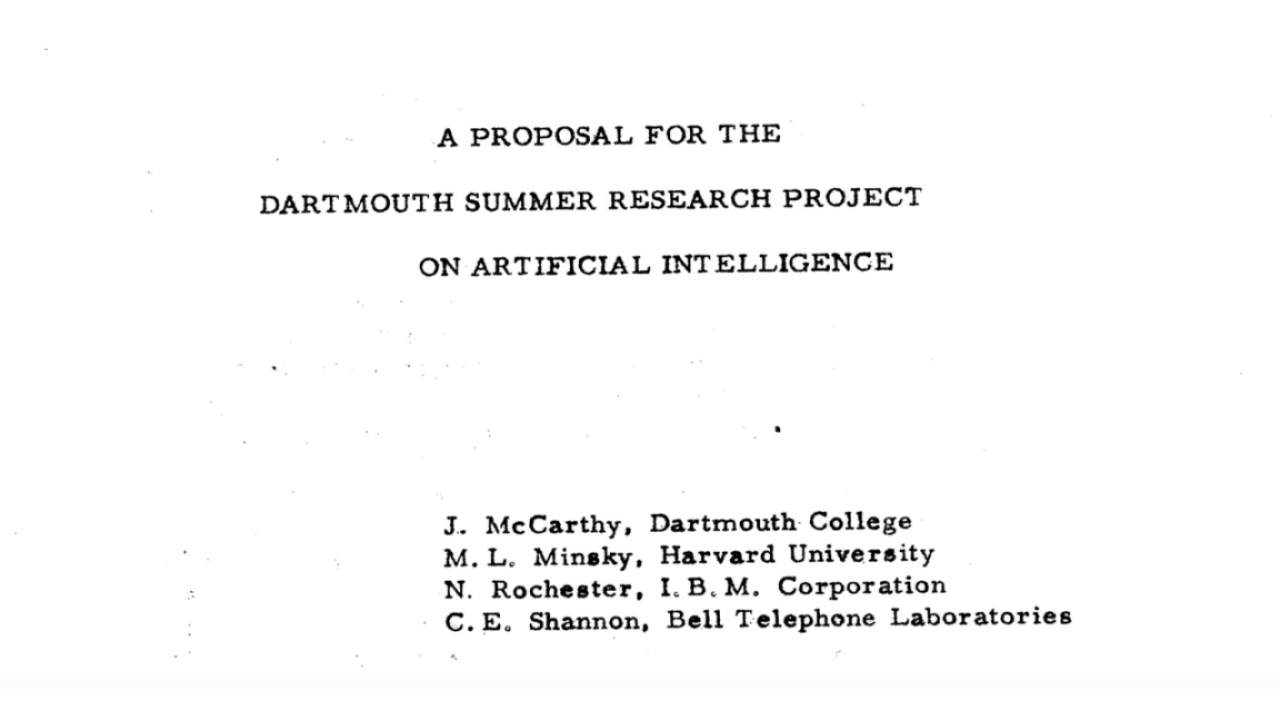
\includegraphics[width=0.75\linewidth]{image/1/artificial-intelligence.png}
	\caption{麦卡锡提交的提议《达特茅斯夏季人工智能研究项目提案》}
\end{figure}


1956 年夏季，在美国新罕布什尔州汉诺威镇的达特茅斯学院召开的会议，是人工智能发展史上的关键转折点，具有不可磨灭的标志性意义，被视为这一领域的重要里程碑。此次会议由约翰・麦卡锡、马文・明斯基、克劳德・香农和纳撒尼尔・罗切斯特四人牵头发起并负责筹备组织工作。他们凭借自身在学术界和科研领域的影响力与号召力，吸引了来自多个不同领域的十余名顶尖专家学者。这些领域涵盖数学、计算机科学、神经心理学、认知心理学以及信息论等，参会人员均在各自专业领域拥有深厚造诣和丰富经验，代表了当时科学界在相关领域的前沿水平。


会议进程中，专家学者们围绕智能机器的理论与实践展开了深入且细致的探讨与交流。在经过多轮严谨的论证和思维碰撞后，首次明确提出了 “人工智能” 这一术语，这不仅仅是一个名称的确定，更是对一个全新研究领域的精准定位。他们从学术层面深入剖析了人工智能所涉及的理论体系，包括但不限于逻辑推理、知识表示、机器学习等核心理论分支，并详细规划了这些理论在实际应用中的方向和场景，如工业自动化生产中的智能控制系统、医疗诊断领域的辅助决策系统以及交通运输中的智能调度系统等，清晰界定了其研究范畴。同时，确立了人工智能的发展目标，旨在创造出能够模拟人类智能行为，甚至在某些特定任务上超越人类智能的机器系统，通过构建基础理论框架，为后续的研究工作提供了系统性的指导原则和方法路径。这一系列成果标志着人工智能成功摆脱萌芽期的混沌无序状态，正式作为一门独立学科登上了科学技术的历史舞台，引发了科学界、产业界以及社会各界对这一新兴领域的广泛关注和探索热情，从而拉开了人工智能第一个热潮的序幕。


在这一发展阶段，符号主义成为人工智能研究的主流方向。符号主义的核心观点认为，世界万物的实体、抽象概念以及它们之间存在的相互关系，均能够通过特定的符号进行准确表示。基于这一理念，计算机可以对这些符号进行逻辑推理和问题求解操作，以实现智能行为模拟。在此理论框架下，研究工作取得了多项具有开创性的初步成果。艾伦・纽厄尔和赫伯特・西蒙开发的逻辑理论家，作为人工智能早期的重要成果之一，能够运用逻辑推理规则对数学定理进行证明，这在当时展示了计算机在处理复杂逻辑问题上的潜力，为后续更高级的智能推理系统开发提供了重要的技术思路和方法借鉴。通用问题求解器的出现则进一步引入了启发式搜索概念，通过对问题空间的智能搜索策略，提高了计算机解决复杂问题的效率和能力，使得人工智能在逻辑推理与问题解决方面向实用化迈进了重要一步。


在语言处理领域，早期机器翻译研究也开始起步。尽管受到当时技术条件的诸多限制，如语言规则的复杂性、词汇语义的多样性以及不同语言文化背景差异等因素影响，翻译成果的准确性和流畅性有限，但这一探索为后续机器翻译技术的发展积累了宝贵的实践经验，包括语言数据的收集与整理方法、语法和语义分析模型的构建思路以及翻译算法的优化方向等。约瑟夫・魏泽鲍姆开发的 ELIZA 程序在自然语言处理与人机对话技术方面取得了初步进展，该程序能够模拟简单的对话场景，对用户输入的自然语言文本进行一定程度的理解和回应，虽然其对话能力还较为初级，但为后续更加智能和复杂的人机对话系统开发奠定了基础。与此同时，计算机在其他领域也展现出了初步的智能应用能力，例如能够解决代数应用题，通过对数学问题的理解和算法运算得出正确答案；能够证明几何定理，运用几何知识和推理规则完成定理的证明过程；还能够学习和使用英语，包括词汇的记忆、语法的运用以及简单文本的理解和生成等功能，这些成果在当时极大地激发了人们对人工智能未来发展的想象空间。


1965 年，爱德华・费根鲍姆成功开发出首个专家系统 DENDRAL，这一成果在人工智能的发展进程中具有重要的标志性意义。DENDRAL 系统专注于化学领域，通过整合该领域丰富的专业知识和大量的实践经验，构建了完善的知识库和高效的推理机制，能够有效地模拟人类专家在分子结构鉴定方面的决策过程。具体而言，它能够依据质谱数据所提供的分子碎片信息，运用知识库中的化学知识和推理规则，准确推断出分子的结构组成，这一应用极大地提高了化学研究中分子结构鉴定的效率和准确性，为后续专家系统在各个不同专业领域的广泛开发和应用提供了成功范例和技术基础，推动了专家系统这一重要人工智能分支的蓬勃发展。


同样在这一时期，1957 年弗兰克・罗森布拉特发明的感知机作为早期神经网络模型的重要代表，为机器学习和人工智能的长远发展提供了关键的基础支撑。感知机模型基于神经元的基本结构和工作原理，通过对输入数据的加权处理和阈值判断，实现对简单模式的识别和分类功能，为后续神经网络技术的发展提供了最初的理论和实践模型。1959 年，萨缪尔提出 “机器学习” 这一具有深远影响的术语，并通过开发会下跳棋的计算机程序对该概念进行了成功验证。这个程序创新性地采用自学习策略，基于 “启发式搜索” 不断优化下棋决策过程。在与跳棋冠军的实际对弈中，通过不断学习和改进自身的下棋策略，展现出超越普通玩家的水平，这一成果充分证明了计算机通过学习能够提升自身智能水平的可能性，为机器学习领域的后续发展指明了方向。


然而，任何技术的发展都难以避免受到时代背景和技术条件的限制。在人工智能发展的初期，当时的计算能力和数据量成为了制约其进一步发展的关键瓶颈。计算机的运算速度和存储容量相对有限，无法满足复杂人工智能算法对大量数据处理和快速运算的需求。许多早期的人工智能方法在尝试处理复杂实际问题时遇到了重重困难，难以达到预期的效果。例如在复杂图像识别领域，由于计算能力不足，无法对高分辨率图像中的大量像素信息进行快速有效的特征提取和模式识别，导致图像识别的准确率和速度都难以满足实际应用的需求；在自然语言语义理解方面，由于缺乏大规模的语料库数据支持和强大的计算能力来进行语义分析和上下文推理，计算机往往只能理解简单的语句结构和字面意思，对于复杂的语义关系、隐喻、歧义等语言现象的处理能力十分有限，进展缓慢。这些问题使得人工智能研究逐渐陷入困境，曾经对这一领域充满热情的投资方和政府机构，由于看不到短期内的实际应用成果和经济效益，逐渐减少了资金支持力度，导致人工智能的第一个热潮逐渐消退。


尽管如此，这一时期的研究成果依然在人工智能的发展长河中具有不可忽视的重要地位。这些早期的探索和实践为后续人工智能的发展积累了丰富而宝贵的经验和教训，无论是成功的技术思路和方法，还是失败的尝试和遇到的问题，都为后来的研究者提供了重要的参考依据和借鉴方向。这些成果奠定了人工智能发展的坚实基础，在学术理论、技术实践以及人才培养等多个方面都产生了深远的影响，引导着后续研究在曲折中不断前行，朝着更加深入、更加有效的方向持续发展，为人工智能在未来的突破和腾飞积蓄了力量。



\subsection{人工智能的第二个热潮}


20 世纪 80 年代至 90 年代，人工智能迎来了第二次热潮，这一时期专家系统的兴起成为主要驱动力之一。专家系统专注于特定领域知识的精准表示与严密推理，其核心在于精心构建知识库和推理引擎。例如在医疗诊断领域，它能够依据大量的医学知识和临床经验，对患者的症状、检查结果等信息进行综合分析，从而辅助医生做出更准确的诊断；在化学分析方面，像卡耐基梅隆大学为美国数字设备公司开发的专家系统 xcom，在 7 年间为该公司节约了 4000 万美元，它能够对化学数据进行有效解读，优化生产流程，这一显著的经济效益引发了全球范围内开发和部署专家系统的浪潮，充分展现出人工智能在实际场景中的应用价值。


与此同时，语音识别技术也取得了重要突破，成为这一时期最具代表性的成果之一。其突破的关键在于大胆放弃了符号学派的传统思路，转而采用统计思路来解决实际问题。这种转变使得语音识别系统能够更好地应对现实中的各种语音变化和不确定性，通过对大量语音数据的统计分析，精准地识别语音内容，从而使语音识别的准确率和实用性得到了大幅提升，为后续智能语音交互的蓬勃发展奠定了坚实基础，如智能语音助手的初步应用，开始改变人们的生活和工作方式。


然而，专家系统虽然在特定领域取得了成功，但也暴露出诸多问题。在知识获取方面，需要耗费大量的人力、物力和时间去收集、整理领域知识，且往往依赖于领域专家的经验，知识的获取过程艰难且效率低下；在维护上，随着知识的快速更新和领域的动态变化，知识库的维护变得复杂且成本高昂；此外，面对复杂多变的现实情况，专家系统难以处理不确定性问题，其推理能力受到很大限制。这些问题使得专家系统的应用范围逐渐受限，随着其他技术的不断发展，其优势逐渐减弱，人工智能研究再次陷入低谷。


在这一时期，众多重要人物及其研究成果为人工智能的发展添砖加瓦。约翰・霍普菲尔德于 1982 年构建了一种新的全互联的神经元网络模型，具有自联想记忆和异联想记忆的功能，为神经网络的发展开辟了新方向，其研究成果对认知科学和人工智能领域产生了重要影响，代表作是《视觉计算理论》。大卫・鲁梅尔哈特推广了 “反传法” 的神经网络训练方法，极大地提升了神经网络的训练效率，使得多层神经网络的训练变得更加可行和高效，推动了神经网络在人工智能领域的广泛应用和深入发展，其代表作是与 “反传法” 神经网络训练方法相关的研究。道格拉斯・勒纳特从事机器学习、知识表示等研究，其博士论文《数学中发现的人工智能方法 —— 启发式搜索》描述了名为 “AM” 的程序，该程序能在大量启发式规则的指导下开发新概念数学，为人工智能在知识发现和概念形成方面的研究提供了有益的探索路径。


这一时期还发生了许多具有影响力的大事件。1980 年，卡耐基梅隆大学为美国数字设备公司成功开发专家系统 xcom，引发全球开发热潮；1981 年，日本政府拨款 8.5 亿美元打造第五代计算机，旨在发展能像人类一样对话、翻译、处理图片、推理的机器，虽然后期计划失败，但反映了当时全球对人工智能发展的高度期望；1982 年，物理学家 John Hopfield 展示新型神经网络，同年 David Rumelhart 推广 “反传法”，双双推动了技术进步；1984 年启动的大百科全书（cyc）项目，试图将整个人类知识装进计算机，让人工智能像人类一样推理，虽未完全实现，但激发了更多关于知识表示和推理的研究；1987 年，苹果和 IBM 生产的台式机性能超过 Symbolics 生产的昂贵 lisp 机，使得专家系统的光环开始褪色；1991 年日本第五代计算机计划失败，1993 年人工智能领域经历信任危机，人们开始反思并尝试强化学习、模仿学习等自下而上的学习方式，推动了人工智能研究方向的转变。


此外，还有其他重要人物及其成果。汉斯・贝利纳打造的计算机程序战胜双陆棋世界冠军；兰德・戴维斯在斯坦福大学获得人工智能博士学位后，发表文章提出使用集成的面向对象模型来提高知识库开发、维护和使用的完整性；大卫・马尔 1982 年发表的《视觉计算理论》对认知科学影响深远；朱迪亚・珀尔倡导人工智能的概率方法和贝叶斯网络，为后来的因果推断奠定基础；罗德尼・布鲁克斯提出更直接、更自然的智能形式，强调通过感知和与环境的互动来实现智能行为；格瑞・特索罗打造的自我学习双陆棋程序，为增强学习的发展奠定了基础。


在学术成果方面，多层神经网络和反向传播算法取得突破，1982 年约翰・霍普菲尔德构建的全互联神经元网络模型，以及 1986 年 Rumelhart 构建的反向传播学习算法（BP），成为普遍应用的神经网络学习算法。1975 年马文・明斯基提出框架理论用于知识表示，1976 年大卫・马尔提出视觉计算理论并由学生归纳总结成书。1976 年兰德尔・戴维斯发表文章提出提高知识库开发、维护和使用完整性的方法。1979 年卡耐基梅隆大学为 DEC 公司制造的专家系统可节约大量费用。1980 年德鲁・麦狄蒙和乔恩・多伊尔提出非单调逻辑。罗德尼・布鲁克斯等人推动了基于行为的机器人学快速发展。1985 年，朱迪亚・珀尔首先提出贝叶斯网络。这些成果共同构成了这一时期人工智能发展的丰富画卷，为后续的研究和应用积累了宝贵的经验和技术基础，尽管经历了起伏，但依然推动着人工智能在曲折中不断前进，探索更加广阔的发展空间。


\subsection{人工智能的第三个热潮}


20 世纪 90 年代至今，人工智能迎来了第三次浪潮，这次浪潮展现出前所未有的活力和影响力，深刻地改变着社会的方方面面，推动人类进入智能时代。


1990 年以来，计算能力的大幅提升和数据量的爆炸式增长成为人工智能发展的重要基石。新型人工智能芯片的不断演进，如 GPU 的广泛应用以及各类专为人工智能优化的芯片架构的出现，结合云计算技术的强大支撑，使得计算机能够处理海量的数据和复杂的计算任务，为大规模神经网络模型的训练提供了坚实的硬件保障，极大地加速了人工智能技术的发展进程。


1998 年，Y. LeCun 提出的卷积神经网络（Convoluted Neural Network），成为深度学习领域的经典算法之一，在图像识别等领域展现出卓越的性能，为后续深度学习算法的发展和应用奠定了基础。进入 21 世纪，机器学习和深度学习逐渐成为人工智能研究的主流方向，并在各行业中得到了广泛的应用，推动了行业的智能化升级。2001 年，William Cleverland 提出的数据挖掘概念，进一步拓展了人工智能在数据处理和知识发现方面的应用范畴。


2006 年是深度学习发展史上的关键转折点。杰弗里・辛顿发表了《一种深度置信网络的快速学习算法》，与此同时，其他重要的深度学习学术文章也相继问世，在基本理论层面取得了一系列重大突破，掀起了人工神经网络的第三次浪潮，为深度学习的广泛应用和深入发展打开了大门，使得神经网络能够更高效地学习和处理复杂的数据模式，从而在图像识别、语音识别、自然语言处理等多个领域取得了显著的成果和进步。


互联网的普及和信息技术的飞速发展，催生了海量数据的产生和积累。社交媒体、电子商务、物联网等领域每天都产生着数以亿计的数据，这些丰富多样的数据为人工智能模型的训练提供了充足且多样化的素材。例如，在图像识别领域，大规模的图像数据集如 ImageNet 的出现，使得深度学习模型能够学习到丰富的图像特征，从而在图像分类、目标检测等任务上不断刷新准确率记录；在自然语言处理领域，海量的文本数据让语言模型能够更好地理解和生成人类语言，推动了机器翻译、文本生成、问答系统等应用的发展。


计算能力的提升与数据的增长相辅相成。一方面，强大的计算能力使得数据的处理和分析更加高效，能够快速完成大规模数据的预处理、模型训练和优化；另一方面，丰富的数据又为计算资源的充分利用提供了广阔的空间，促使研究人员不断探索更复杂、更强大的人工智能模型。这种良性循环推动了人工智能技术在各个细分领域的巨大进步，使得人工智能系统的性能和智能水平得到了质的飞跃，能够更好地应对现实世界中的复杂任务和挑战。


近年来，以 ChatGPT 为代表的 AIGC（人工智能生成内容）技术异军突起，成为人工智能领域的又一热点和亮点。AIGC 在内容创作成本、创作效率、模型计算消耗以及用户流量基础等多个维度实现了重大突破。与传统的内容创作方式相比，AIGC 能够利用深度学习模型快速生成高质量的文本、图像、音频、视频等各种类型的内容，大大降低了创作门槛和成本，提高了创作效率，同时也满足了用户日益多样化的内容需求。


AIGC 的应用前景极为广阔，涵盖了搜索引擎、艺术创作、影音游戏、金融、教育、医疗、工业等众多领域。在搜索引擎方面，它能够为用户提供更加精准、个性化的搜索结果和答案，提升搜索体验；在艺术创作领域，帮助艺术家生成创意灵感、辅助绘画、音乐创作等；在影音游戏中，用于生成虚拟角色、场景、剧情等，增强游戏和影视作品的吸引力和沉浸感；在金融领域，辅助风险评估、投资决策等；在教育领域，实现个性化教学、智能辅导等；在医疗领域，辅助疾病诊断、药物研发等；在工业领域，优化生产流程、进行质量检测等。AIGC 的兴起有望大幅加速 AI 的商业化进程，为各行业带来新的增长点和创新机遇，推动整个社会经济的发展和变革。


在这一次人工智能浪潮之下，也有很多研究学者做出了巨大贡献，他们的研究成果与创新实践成为推动人工智能迅猛发展的关键力量，在全球范围内产生了深远的学术与产业影响。杰弗里・辛顿，作为 “AI 教父”“深度学习之父”，其学术生涯成就斐然。早在 1977 年博士论文中对视觉系统假设处理方法的研究，便为计算机视觉和模式识别奠定理论根基，引领该领域新方向。后续在 1998 年当选英国皇家学会会士，2006 年提出深度信念网络，2012 年取得计算机视觉突破性成果，以及 2018 年荣获图灵奖和 2024 年斩获诺贝尔物理学奖等一系列荣誉，彰显了他在深度学习理论与应用上的卓越贡献，深刻影响着全球人工智能的发展轨迹，其研究成果堪称行业标杆。Yann LeCun 同样贡献卓越，在深度学习和神经网络领域建树颇丰。自 1983 年获得巴黎 ESIEe 电气工程师文凭后持续深耕，1987 年取得博士学位，凭借对卷积网络模型在计算机视觉与语音识别等应用的深入钻研而声名远扬。他发表 200 余篇学术论文，涉及多领域，推动技术实际落地。2018 年图灵奖的获得以及著作的发表，为人工智能学术与实践提供关键指引，促进了产业发展与技术进步。吴恩达 2002 年加入斯坦福大学创立实验室后，积极开展前沿研究，率先将 GPU 应用于深度学习，极大提高训练效率，推动技术普及。此后创立 “谷歌大脑” 与领导 “百度大脑” 项目，联合创立 Coursera 并创建相关教育机构，在学术研究、人才培养与产业应用方面均成果显著。其数百篇论文与众多荣誉，见证了他在全球人工智能领域的广泛影响力。李开复 1988 年以开创性的博士论文成果开启其辉煌历程，在多家全球顶尖科技公司任职积累深厚经验后，回国创建微软中国研究院，助力中国计算机技术发展；后创立创新工场扶持人工智能初创企业，2023 年筹组 project AI2.0 并推出优异大模型，彰显中国人工智能实力，在全球领域崭露头角。戴米斯・哈萨比斯和约翰・江珀 2024 年荣获诺贝尔化学奖，他们的 AlphaFold 技术通过融合实验数据与机器学习算法，精准预测蛋白质三维结构，为生命科学与生物技术领域带来革命性突破，充分展现人工智能在交叉学科的巨大潜力，推动了人类健康事业的进步，进一步拓展了人工智能的应用边界与价值。这些学者的杰出贡献共同编织了当代人工智能蓬勃发展的壮丽篇章，为后续的探索与创新铺就坚实道路，持续激励着全球科研人员不断攀登人工智能的新高峰，推动这一领域向着更高水平、更广泛应用的方向稳步迈进。


综上所述，第三次人工智能浪潮在技术突破、数据利用、计算能力提升、新兴技术兴起以及关键人物的推动下，正以前所未有的速度和深度改变着世界，为人类社会的发展带来了无限的可能和机遇，同时也面临着一些技术、伦理和社会等方面的挑战，需要我们在追求技术进步的同时，积极应对和解决这些问题，以实现人工智能的可持续发展和造福人类的最终目标。


\section{人工智能的现状}


步入 2020 年代，人工智能大模型以燎原之势火爆全球，AIGC（人工智能生成内容）更是掀起了一波又一波的新热潮，公众对人工智能的关注度与日俱增，其已成为全球科技与产业发展中一股不可或缺的重要力量，一个充满无限可能与活力的人工智能时代正快步向我们走来。


在诸多领域，人工智能都展现出了强大的影响力和应用潜力。在医疗健康领域，它助力疾病的精准诊断，通过对海量医疗影像数据的学习和分析，能够快速、准确地识别出病症特征，为医生提供辅助诊断建议，大大提高诊断效率和准确性；在交通出行方面，无人驾驶技术不断取得突破，智能交通系统可以优化交通流量，减少拥堵，提升出行的安全性和便捷性；工业制造中，智能机器人和自动化生产线能够实现高精度、高效率的生产作业，降低人力成本，提高产品质量和生产效率；教育领域，智能辅导系统可以根据学生的学习情况和特点，提供个性化的学习方案和辅导，实现因材施教。


但是随着人工智能的深入发展，其伦理道德问题日益凸显。人工智能模型的不可解释性成为一大困扰，许多复杂的模型决策过程犹如 “黑箱” 操作，难以被清晰解读。这种不可解释性可能对人们长期以来形成的道德伦理观念造成强烈冲击，引发一系列关于责任界定、公平性以及隐私保护等方面的伦理争议。以无人驾驶汽车为例，一旦发生事故，很难明确界定是算法的失误、硬件的故障，还是其他外部因素导致，从而在责任认定上陷入困境。此外，在招聘、贷款审批等场景中，如果基于人工智能算法做出决策，可能会因为数据偏差或算法偏见而产生不公平的结果，对某些群体造成歧视。同时，人工智能系统在数据收集和使用过程中，也可能会侵犯个人隐私，如过度收集用户信息等。因此，迫切需要建立一套全面、完善且具有前瞻性的伦理规范和法律法规，来引导和约束人工智能的发展与应用，确保其符合人类的道德伦理标准和社会价值取向。


人工智能行业的快速发展使得高端复合型人才的需求急剧攀升，然而目前人才培养体系尚不完善，难以满足这一旺盛需求。人工智能领域不仅要求从业者具备深厚的数学、统计学、计算机科学等专业知识，还需要对特定应用领域有深入了解，如医疗、金融、交通等。但现有的教育体系在课程设置和实践教学方面，与人工智能产业的实际需求存在一定程度的脱节，导致高端人才的供给严重不足。这不仅制约了企业的技术创新和产品研发能力，也在一定程度上阻碍了整个行业的健康、快速发展。尽管人工智能技术前景广阔，但众多人工智能企业却面临着盈利困境。一方面，技术研发需要投入大量的资金、人力和时间成本，从算法研究、模型训练到硬件设备的升级，每一个环节都需要持续不断的高额投入。另一方面，将人工智能技术应用落地同样成本不菲，包括适配不同场景的定制化开发、与现有业务系统的集成、数据的收集与整理等。而且，在市场竞争激烈的环境下，许多企业还处于探索商业模式和市场定位的阶段，尚未找到稳定、可持续的盈利途径，这使得大部分人工智能企业在财务上承受着巨大压力，甚至处于亏损状态。


部分人工智能应用领域的法律规制存在明显的缺失或滞后现象。以无人驾驶为例，随着技术的逐渐成熟和应用场景的不断拓展，相应的法律法规却未能及时跟上。在无人驾驶汽车的上路标准、事故责任认定、保险政策等方面，目前还缺乏明确、详细且具有可操作性的法律规范，这使得无人驾驶技术在推广和应用过程中面临诸多不确定性和潜在风险。构建完善的立法体系面临着诸多挑战，如技术的快速更新换代使得法律难以跟上步伐，不同国家和地区的法律差异也增加了协调统一的难度，而且立法者需要在鼓励创新和保障安全、权益之间找到精准的平衡，这无疑是一项艰巨而复杂的任务。


在开源开放的生态建设方面，人工智能也面临着诸多难题。开源对于人工智能技术的快速传播和广泛应用具有重要意义，但目前开源生态存在着技术被抄袭、维护更新不足等问题。一些开发者或企业在使用开源代码后，未遵循开源协议进行回馈和维护，导致开源项目的可持续性受到威胁。此外，开源社区的管理和协作机制也有待进一步完善，以提高代码质量和安全性，促进技术的迭代升级和广泛应用。


如前文所述，人工智能模型的不可解释性不仅是技术问题，更是科技伦理问题。从长远来看，需要从技术和法律两个层面加以限制和规范。在技术层面，研究人员应致力于开发可解释性强的人工智能算法和模型，通过可视化技术、特征选择方法等手段，让模型的决策过程更加透明和易于理解。在法律层面，应制定严格的法规，明确要求人工智能系统的开发者和使用者对模型的决策机制进行说明和备案，确保其符合伦理道德和法律要求。同时，在应用设计上，应改变单纯追求效率和准确性的逻辑，将人类价值观和道德标准融入其中，使人工智能成为人类发展的有益补充，实现与人类的和谐共生、共赢发展。


人工智能自身存在着诸多安全风险。算法模型的可解释性不足不仅引发伦理问题，也对系统的安全性构成威胁，难以察觉和修复潜在的算法漏洞和偏差。框架安全漏洞可能被黑客利用，导致系统被攻击、数据被窃取或篡改。数据标注作为人工智能训练的重要基础，如果存在不规范问题，如标注错误、标注信息不完整或存在偏差，会影响模型的准确性和可靠性，进而引发一系列安全隐患。这些问题都严重影响了人工智能系统的可信度和稳定性，制约了其在关键领域的广泛应用和深入发展。


对个人和组织而言，人工智能可能带来隐私泄露风险，如智能设备收集的个人数据被非法获取；生命安全风险，如恶意利用医疗人工智能设备干扰正常治疗；财产损失风险，如网络诈骗借助人工智能技术手段更加隐蔽和难以防范；伦理道德风险，如利用人工智能合成虚假信息误导公众。从国家和社会层面看，在政治领域，人工智能可能被用于操纵选举、传播虚假政治信息；文化方面，可能导致文化多样性受到冲击，本土文化被侵蚀；经济领域，可能加剧市场垄断，破坏公平竞争环境；军事领域，自主武器系统的失控可能引发不可估量的后果。从全人类角度出发，人工智能的大规模训练和应用，如 GPT 等模型的训练，消耗大量能源，导致资源浪费和碳排放增加，对地球的可持续发展构成威胁，且其发展方向和潜在影响在一定程度上存在不可控性。


尽管人工智能在发展进程中面临着数据隐私泄露、算法偏见、安全漏洞等诸多严峻挑战，但全球在人工智能安全治理方面已迈出了坚实步伐，取得了令人瞩目的进展。世界各国经济体深刻认识到问题的紧迫性和严重性，纷纷投身于完善自身人工智能治理体系的建设之中。例如，欧盟制定了《人工智能法案（EU AI Act）》，对人工智能系统进行了分类监管，明确了不同风险等级的系统应遵循的规则和要求，旨在全方位加强对人工智能技术研发、应用推广等各个环节的监管与规范，确保其安全可靠发展，为欧洲地区的人工智能产业营造了严谨的法治环境。美国则通过发布一系列政策文件和指南，如《国家人工智能研发战略计划》等，引导联邦机构在推动人工智能创新的同时，重视安全和伦理问题，强调在关键领域应用人工智能时的风险评估与管理，为其在全球人工智能领域的竞争与发展保驾护航。中国积极出台相关政策和法规，从国家战略高度布局人工智能发展方向，注重发展与安全的平衡，在数据安全、算法治理等方面不断强化规范，推动人工智能赋能实体经济的同时保障社会稳定与公众权益。英国、日本、印度、韩国等国家也各自根据本国国情和发展需求，制定了相应的人工智能政策和立法举措，从不同维度加强对人工智能的治理和引导，如英国的《国家数据战略》为人工智能数据利用提供了框架，日本在机器人伦理等方面的探索为人工智能安全应用提供了有益参考，印度在信息技术领域的传统优势基础上构建人工智能治理规范，韩国在智能产业发展中注重安全标准制定，这些国家的努力共同绘就了全球人工智能安全治理的多元图景。


与此同时，产业组织也充分发挥着协同优势，积极推动人工智能产业的健康发展和安全应用。诸多国际产业联盟和行业协会通过制定统一的行业标准，为企业的技术研发和产品应用提供了规范指引，促进了市场的有序竞争和技术的互通互鉴。例如，电气与电子工程师协会（IEEE）等组织发布的人工智能伦理准则和技术标准，在全球范围内得到了广泛的认可和遵循，有力地推动了行业自律和技术的稳健发展。各大企业更是积极响应安全治理的号召，主动承担起社会责任，开展负责任的研发与应用实践。谷歌设立了专门的人工智能伦理委员会，致力于审查和指导公司的人工智能项目，从算法设计的公正性到数据使用的合理性，都进行严格把关，确保技术的开发和应用符合伦理道德和安全规范；百度在人工智能研发过程中，高度重视数据安全和隐私保护，采用先进的加密技术和访问控制措施，保障用户数据不被泄露和滥用，同时积极探索算法的可解释性，提升人工智能决策的透明度；微软投入大量资源进行人工智能安全技术的研发，通过构建强大的安全防护体系，抵御潜在的网络攻击和恶意利用，为其云服务和各类人工智能产品提供坚实的安全后盾。这些企业的积极作为，不仅提升了自身的品牌形象和市场竞争力，更为整个行业树立了良好的榜样。


然而，必须清醒地认识到，人工智能安全治理是一个长期而复杂的系统性工程，绝非一蹴而就。当前的治理成果仅仅是一个开端，仍需要全球各界持续不断地探索更加行之有效的治理方案。一方面，要进一步完善风险识别方法，借助大数据分析、人工智能监测等先进技术手段，敏锐捕捉潜在的风险信号，提高对诸如深度伪造技术带来的新型风险的敏感度和预警能力，做到防患于未然；另一方面，需不断强化风险评估与防范机制，建立健全涵盖技术、法律、伦理等多维度的综合评估体系，确保在人工智能技术发展的每一个阶段、每一个应用场景中，都能将风险严格控制在可接受的范围内。只有通过全球各国、各产业组织以及企业的共同努力，持之以恒地加强治理与协作，才能为人工智能时代的人类社会构建一道坚不可摧的安全屏障，让人工智能技术真正造福人类，引领人类迈向更加美好的未来。

\section{总结与习题}
总结：本章探讨了人工智能的含义，包括智能的定义和机器能否思考的问题，总结了人工智能基于不同方面的分类，人工智能的三个热潮以及人工智能的现状。


习题：人工智能是在哪一年成为正式学科的？


图灵测试是什么？


2006年为什么是深度学习发展史的分水岭？